%!TEX root = ../final_report.tex

%Introduction, which describes the motivation and goal of your project. Describe how your project is connected to existing literature. Include references to scientific papers that are relevant to your topic. Do not copy your text from the intermediate report. Revise and rewrite according to the feedback you got and what the actual outcome of the project was.

This report presents the system we developed for the Computer Vision Masters Project, the results of our experiments using it and our reflections on the project as a whole.

% The goal for the project was to develop software to allow an autonomous robot to locate objects in its environment.
In order to accomplish even simple tasks such as fetching and carrying, autonomous systems working in human environments must be able to find and interact with objects.
The first step in this process is object detection, where the robot identifies which parts of its environment are likely to correspond to an actual object.
Having identified these areas, a model of object positions and shapes can be built, which the robot can use e.g. to speed up the search for a specific object which it needs to accomplish its current task or to aid navigation and object interaction.

The goal of the project was to develop software which would allow an autonomous mobile system to efficiently create such a model, starting with no prior knowledge of the objects or the environment.
Specifically, we were interested in the next best view (NBV) problem: given the currently available knowledge, where should the robot move to next in order to gain the maximum possible increase in knowledge, and thus biuld its model in the shortest possible time?
The experimental heart of the project was the implementation of several different NBV algorithms and comparing the performance which they achieve.

% When a robot is visiting a place for the first time it might be a good idea to explore this room to create such a list of available objects.
% This is the situation and the task that we want to solve with our system.
% To be able to do this, it is necessary to perform simultaneous localization and mapping, detect potential objects in the current view, and to compute the next best view (NBV) which allows to explore the environment.

% Previously, however, to conclude the introduction we present some existing approaches in the subject of object detection in autonomous robots and then in Section \ref{Theoretical_background} we introduce some of the core methods and concepts used for the implementation of our system.
% In Section \ref{Analysis} we explain the performed experiments and obtained results of them, which allows to access the strengths and weaknesses of the system. In the end Section \ref{Conclusion} concludes this final report with a summary, a short assessment of the changes and learnings we had since the proposal of our project.

In the remainder of this introduction we present first some recent approaches to this problem (section \ref{sub:related_work}) and then a brief overview of the system we developed (section \ref{sub:system_overview}).
The report then introduces some of the core theoretical methods and concepts which we used (section \ref{Theoretical_background}) before detailing our implementation (section \ref{Implementation}).
The results achieved by the system are presented in section \ref{Analysis}, and in section \ref{Conclusion} we conclude the report and offer our reflections on the project.

\subsection{Related work}
\label{sub:related_work}

In \cite{monica2017}, Monica and Aleotti propose a system for model-free NBV planning on a robot arm, using data from a Kinect camera.
They use the concept of contours -- voxels which neighbour both unknown voxels and occupied voxels -- to guide the generation of candidate view poses, and then a saliency heuristic to guide the assessment of those poses.
Their method is unusual in that they operate directly on the point cloud data, which requires a large amount of computational effort.

Blodow et al. \cite{blodow2011autonomous} built an autonomous robot that computes NBV poses to generate a semantic map of kitchen environments.
They focus especially on handles of drawers and doors which the robot could interact with.
NBVs are computed by finding potential poses with high information gain. On the one hand they search for poses at which large amounts of border voxels -- voxels at the border between known and unknown space -- can be seen from; and on the other hand, since their map is generated by merging point clouds from various views, it is also taken into account that a large part of the next best view should contain obstacles that are already part of the map.

\subsection{System Overview} % (fold)
\label{sub:system_overview}

\begin{figure}[ht]
	\begin{center}
		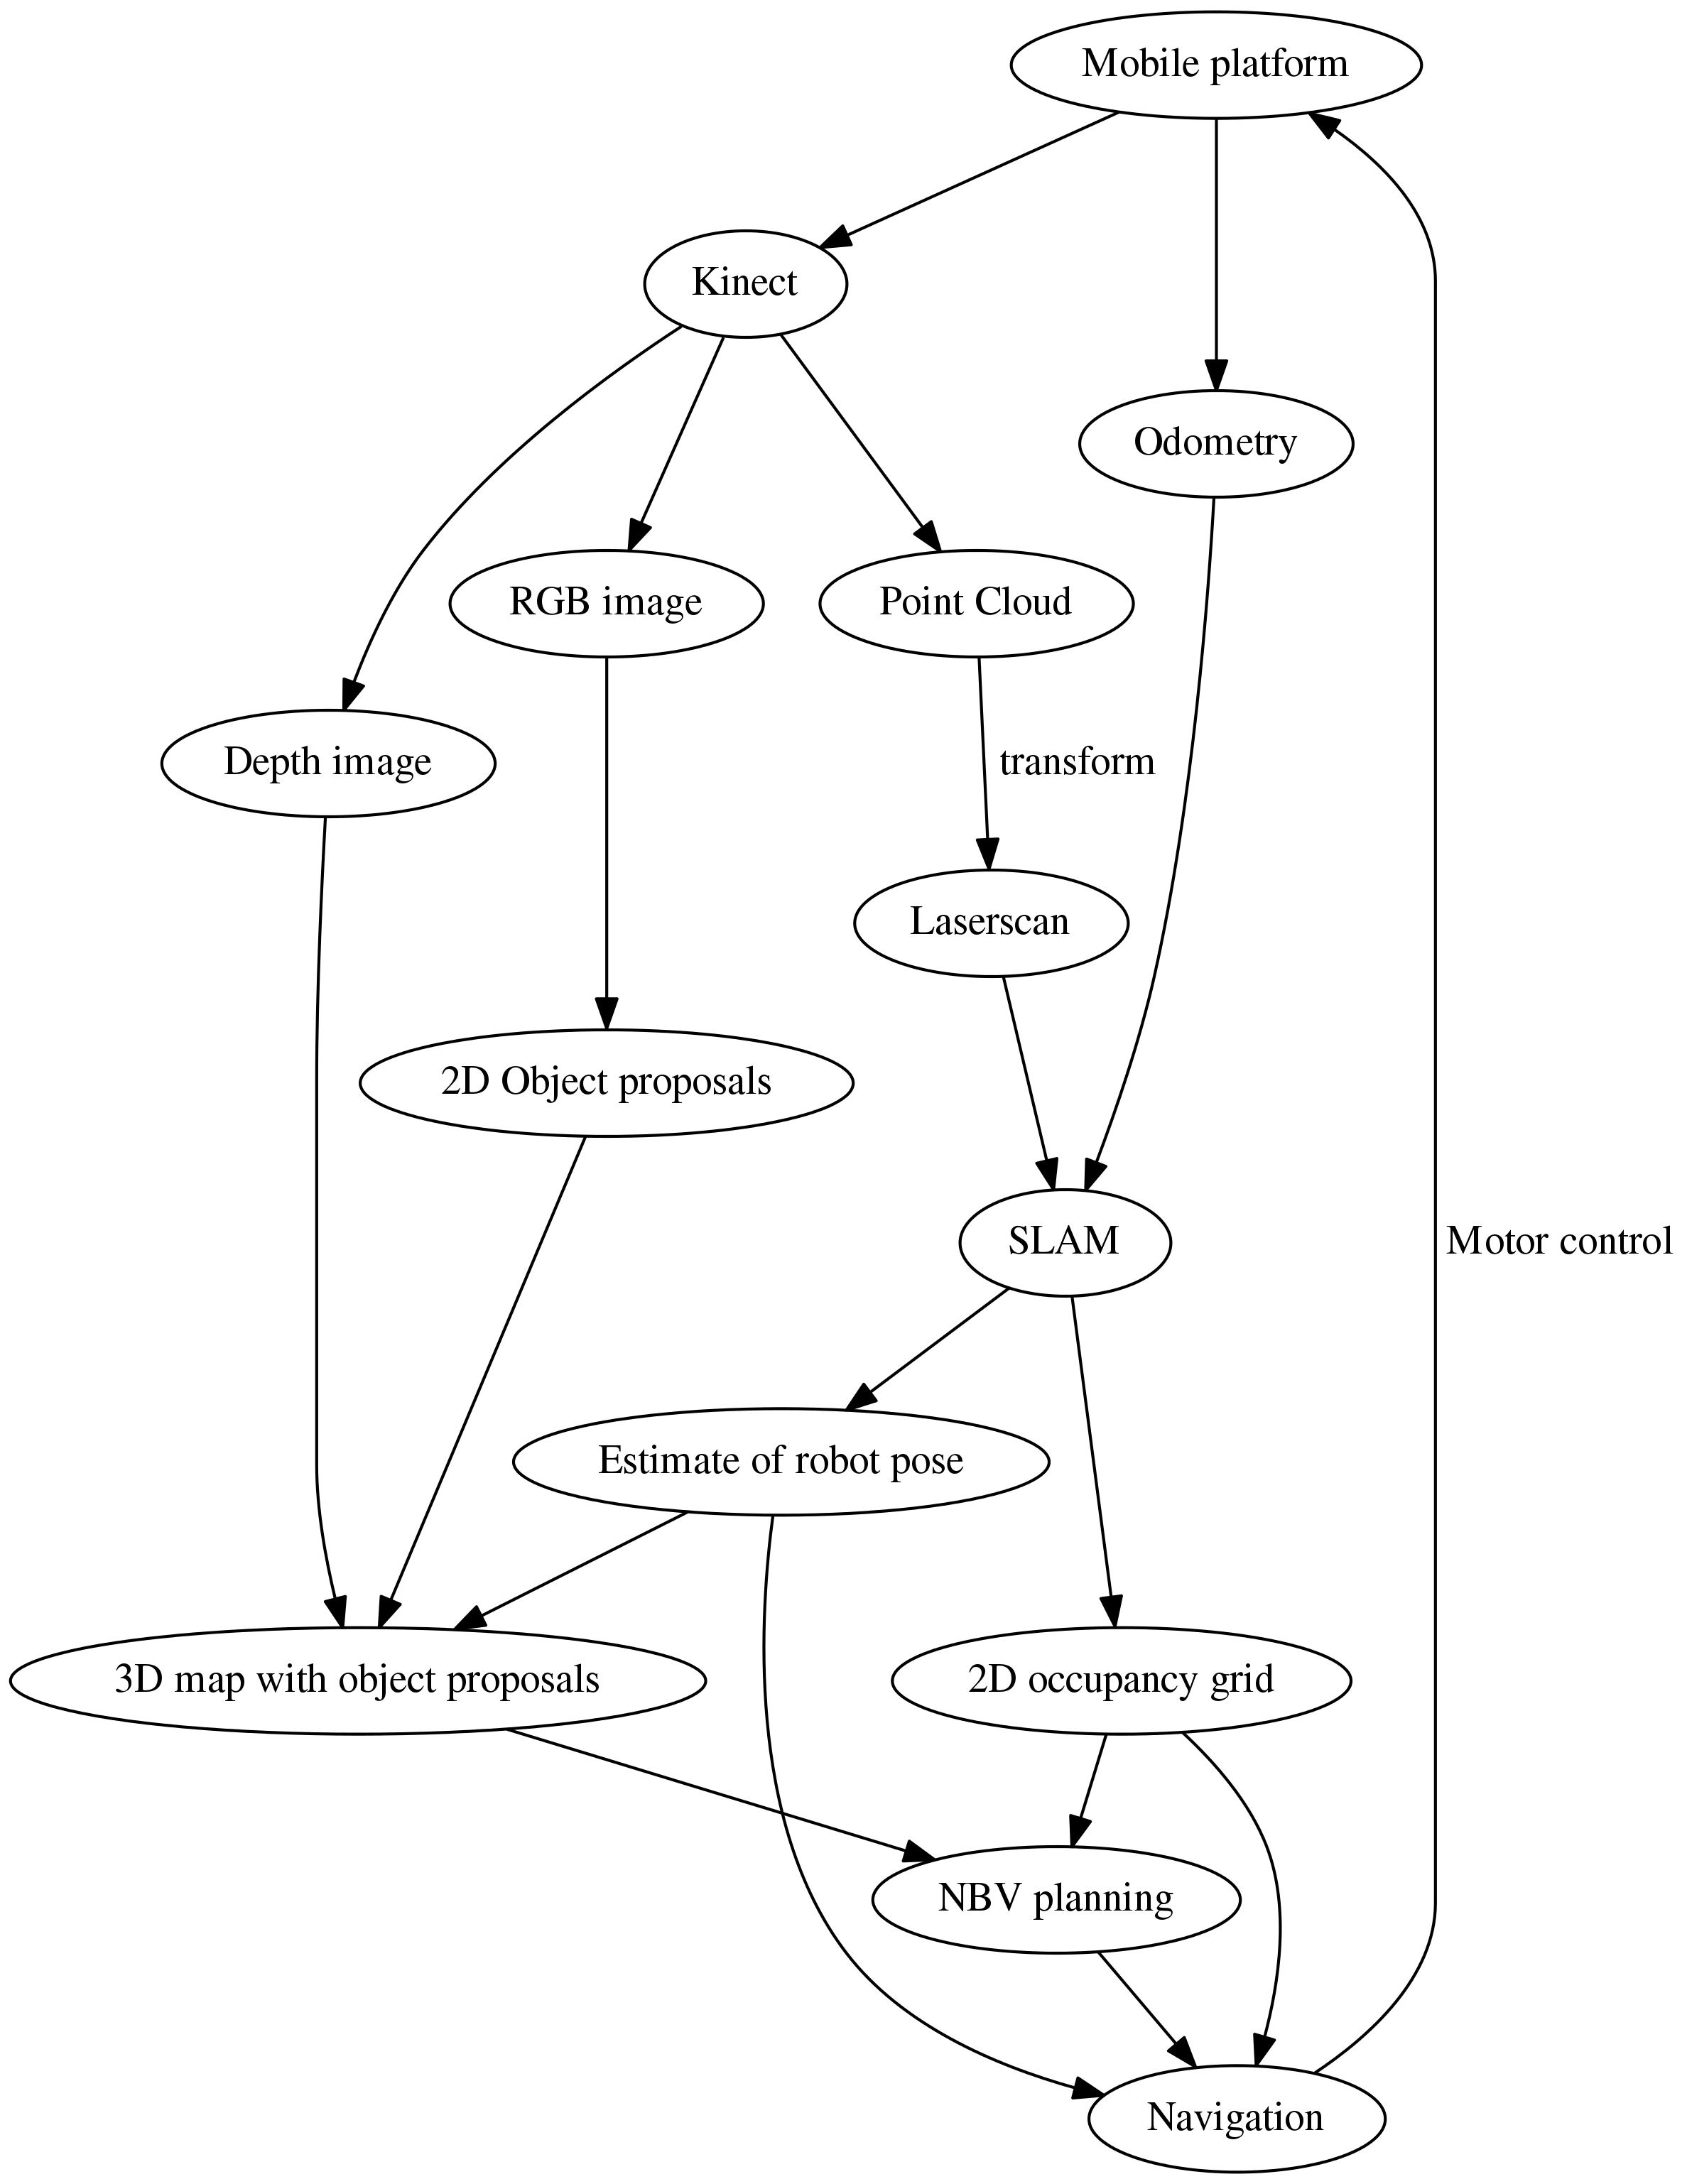
\includegraphics[width=0.85\linewidth]{dot/overview.png} 
		\caption{Overview of the information flow in the system}
		\label{fig:overview}
	\end{center}
\end{figure}

A general overview of the system is given in Figure \ref{fig:overview}.

The input consists of the odometry from the mobile platform and the depth image, colour image, and point cloud data from the mounted RGB-D camera.
Our SLAM algorithm requires laser scan data and the odometry, therefore we transform the point cloud to a simulated laser scan.
The SLAM algorithm provides us with an estimate of the robot's current pose and a 2D occupancy grid: a map of the environment in which each grid cell is set as containing either an obstacle, free space, or unexplored space. 

A new set of object proposals is computed in our system only at each NBV.
Between NBV poses, the camera data is used to improve the map, but not to find further objects.

Our object proposals are at first generated in 2D from the RGB image, then a corresponding point cloud for the object proposal is generated using the available depth information.
This point cloud is further processed to ensure that it represents a contiguous volume.
% To ensure that the object proposal point cloud corresponds to one contiguous volume a clustering algorithm is applied.
% Further processing is done only on the object proposal point cloud cluster closest to the robot. 
The cloud is then projected, with help of the estimated robot pose, into a 3D map, where the new object proposals are merged with already-existing ones.
% 3D object proposals that already have been integrated into the map previously are updated with the new proposals.

We try different NBV algorithms, which can work with the robot's current pose, the 2D map of the environment, and with knowledge about the approximated object positions.
As output of each NBV algorithm we receive the next desired robot pose.
This is then used together with the 2D map and the approximated robot position to navigate the robot.

% A more detailed description of the implementation of the different parts of our system is given in Section \ref{Implementation}.

% subsection system_overview (end)